\documentclass[a4paper, 11pt, twocolumn]{article}
\usepackage[margin=0.8in]{geometry}
\usepackage{xcolor}
\usepackage{graphicx} %package to manage images
\graphicspath{ {./images/} }
\usepackage{amsmath}

\title{AS-06 Mains Power Supplies}
\author{Revision sheet}
\date{}

\usepackage{fancyhdr}
\pagestyle{fancy}
\fancyhead{} % clear all header fields
\renewcommand{\headrulewidth}{0pt} % no line in header area
\fancyfoot{} % clear all footer fields
\renewcommand{\footrulewidth}{0.4pt}
\fancyfoot[C]{\thepage} % page number in centre of the page
\fancyfoot[R]{\footnotesize Thomas Boxall \\ Images from WJEC E-Book} % right hand footer has author name on top line and images reference on bottom line
\fancyfoot[L]{\footnotesize AS-06 Mains Power Supplies \\ Revision sheet} % left hand footer has title of document on top line and 'Revision Sheet' on bottom line

\begin{document}

    \maketitle
\section{Introduction}
\thispagestyle{fancy}
We need a mains power supply to convert from the 240V AC from the wall socket to a lower voltage for devices to use. These could be as low as $\pm5$V DC for a logic system. 

\section{Transformers}
Transformers can step-up the voltage between two coils or step-down the voltage. The equation below links the number of turns and voltages on each coil:\newline
$\frac{V_S}{V_P}=\frac{\mathrm{Number\ of\ turns\ on\ secondary}}{\mathrm{Number\ of\ turns\ on\ primary}}$

\section{Rectification}
AC Voltages have positiver areas and negative areas, we want a single positive voltage. To get that, we have to rectify the AC input.
\subsection{Half-Wave Rectification}
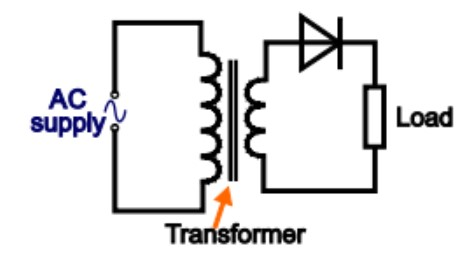
\includegraphics[width=0.4\textwidth]{halfWaveRectificationCD.jpg}\\
The diode only allows current to flow in one direction. The diode has a 0.7V voltage drop across it. \\
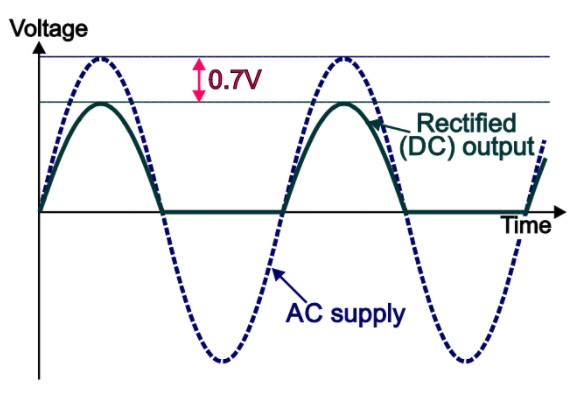
\includegraphics[width=0.4\textwidth]{halfWaveRectificationGraph1.jpg}\\
Half wave rectification wastes 50\% of the power, this isn't great so we can use a full wave rectification circuit instead.

\subsection{Full-Wave Rectification}
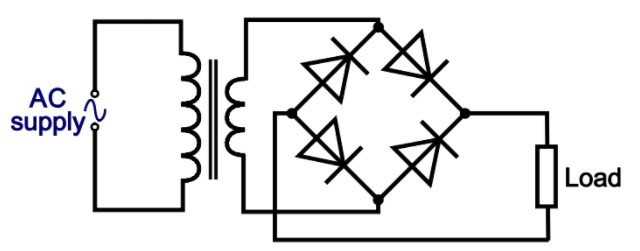
\includegraphics[width=0.4\textwidth]{bridgeCircuit.jpg}\\
This is a bridge rectifier. It works by a positive voltage flowing through two of the diodes and a negative voltage flowing through the other two. As there are two diodes involved this time, there is a 1.4V voltage drop. \\
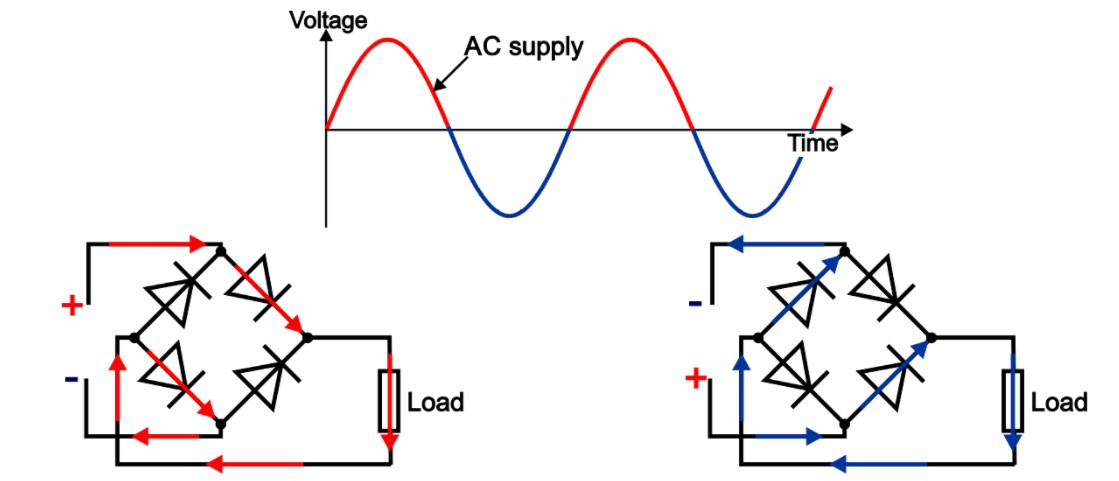
\includegraphics[width=0.4\textwidth]{bridgeCircuitGraph1.jpg}\\
The graph below shows the input and output to the circuit.\\
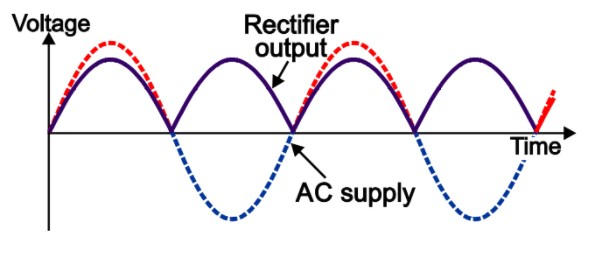
\includegraphics[width=0.4\textwidth]{bridgeCircuitGraph2.jpg}\\

\section{Smoothing}
We want one consistent $V_{out}$, not a bumpy one. To get this, we can use a capacitor to 'smooth' the circuit. This isn't a perfect solution however as we still have a slight drop as the capacitor discharges. This is called the ripple voltage.\\
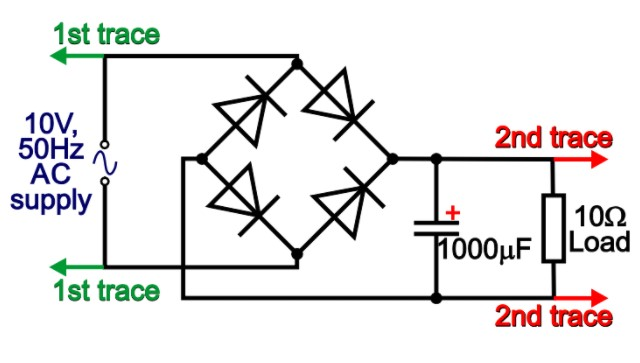
\includegraphics[width=0.4\textwidth]{smoothing1.jpg}\\
The output looks something like this:\\
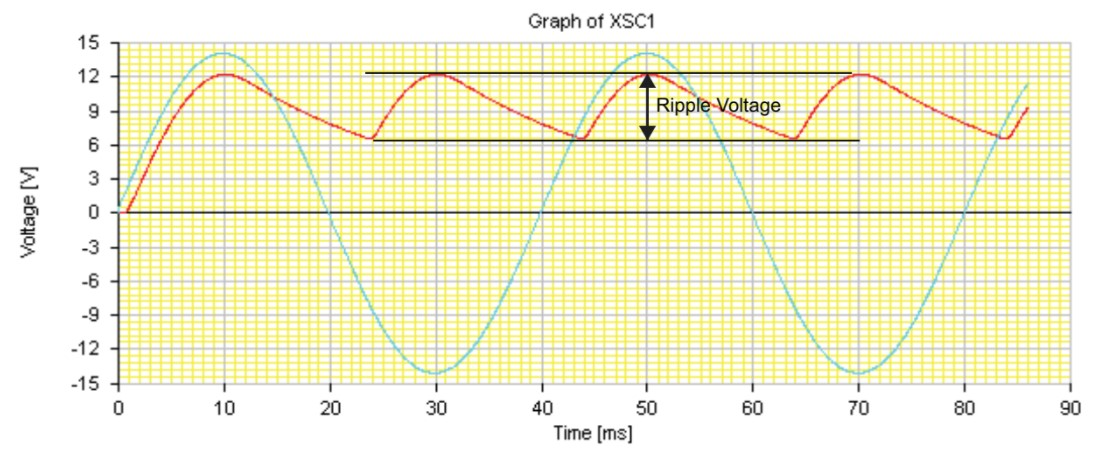
\includegraphics[width=0.4\textwidth]{smoothing2.jpg}

\section{Ripple Voltage}
The ripple voltage can be calculated using the following equation:\\
$\displaystyle V_R = \frac{I_c}{F C}$\\

\section{Regulation}
The output from smoothing can be relatively smooth but it does have some small bumps. We want a perfectly smooth output, at a single constant voltage. To achieve this, we have to regulate the output.\\
Regulation is achieved using a component called a Zener Diode. When it is in reverse bias, the Zener Diode has a specified voltage across it, therefore it can be sued a sa voltage reference. They also require a minimum current to flow through them (called a 'holding current'). \\
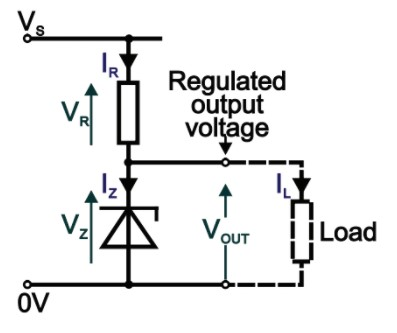
\includegraphics[width=0.4\textwidth]{regulation.jpg}\\
If the load current draw is above the maximum load current which can be provided whilst keeping the zener holding current then the Zener will switch off. 


\end{document}